\documentclass[11pt, a4paper]{report}

\usepackage[english]{babel}
\usepackage[utf8x]{inputenc}
\usepackage{amsmath}
\usepackage[normalem]{ulem}
\useunder{\uline}{\ul}{}
\usepackage{adjustbox}
\usepackage{float}
\usepackage[colorinlistoftodos]{todonotes}

\usepackage{fullpage}
% A more tightly packed list than the standard
% \enumerate{itemize} append * after enumeration type
\usepackage{mdwlist}
% Multi-page tables + accompanying header and footer comments
\usepackage{longtable}

% Vertical table headers, not sure what does what. graphicx is
% multi-purpose and does a lot of other stuff like including images
\usepackage{array,graphicx}
\usepackage{booktabs}

% Lossless .png format expected for figures
\DeclareGraphicsExtensions{.png}

% \verbatiminput command (\begin{verbatim} is standard lib)
\usepackage{verbatim}
% Allows for verbatiminput of files AND breaks lines that are too long
% for the page to fit
\usepackage{listings}

\newcommand*\rot{\rotatebox{90}}

\title{Desi}
\author{Matthew Flickner \\ Loyola Marymount University\\ CMSI402}

% Allow commands
\providecommand\phantomsection{}



\begin{document}

%---    Title page    ---%
\clearpage
\phantomsection
\addcontentsline{toc}{chapter}{%
    \protect\numberline{I}Title Page}
\maketitle


\tableofcontents
\newpage
 
\chapter{1}

\chapter{Original Proposal}
My project for 402 will be called Desi and will be an iOS application built on the Parse SDK. The purpose of Desi is to help a group of people manage their responsibilities. A user of the app belongs to a group with other users. With each group, there are tasks, each of which has a specific user responsible for completing that task. That person is called the Desi. A point is given to the Desi upon completion of his task. Users can volunteer to complete a task if they are not the Desi and earn double points. Points can be used as a payment for the Desi to opt-out of his task.

\chapter{}
 A chapter.

\chapter{}
 A chapter.

\chapter{Software Requirements}

\section{Introduction}
Desi is a system in which a user logs in to create group with other and then create/complete task in a group with those other users. Points are awarded for completing tasks and can be used as currency to opt-out of an assigned task.

\begin{figure}[H]
\centering
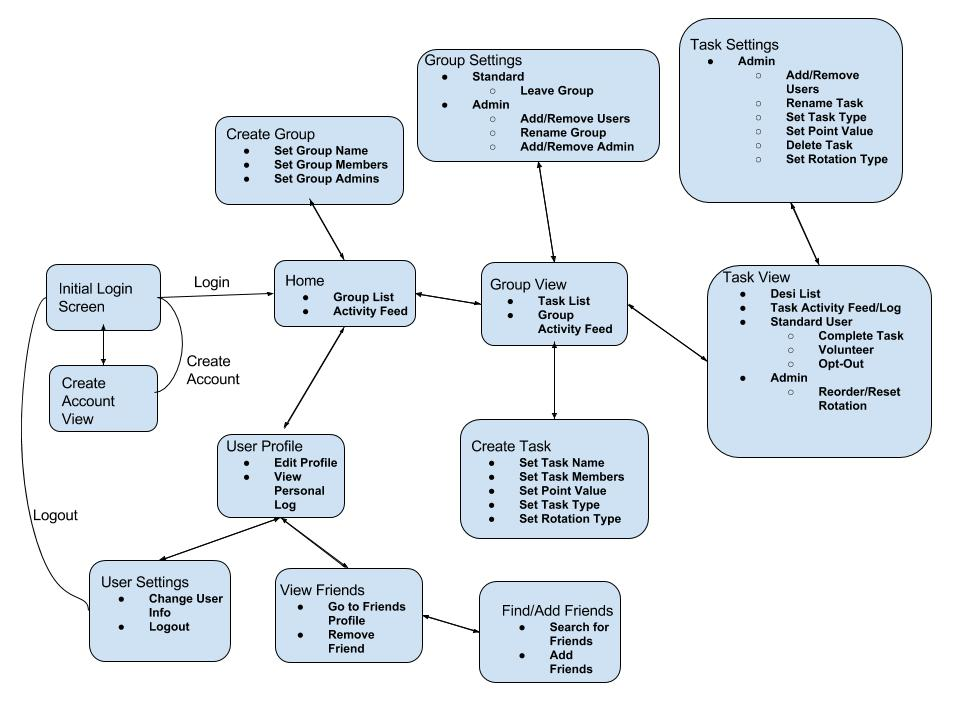
\includegraphics[width=1.0\textwidth]{umlHighLevel.jpg}
\end{figure}

\section{Functional Requirements}
\subsection{General}
\subsubsection{Run on an iOS Device}
Desi must be able to run on a device running iOS.
\subsubsection{Make network calls to the backend}
Desi must be able to make network calls to retrieve or save data.
\subsubsection{Persistant Data}
Desi must make use of the mySQLite iOS datastore to make user data persistent.
\subsubsection{Handle Network Errors}
Desi must be able to function if 

\subsection{Standard User Requirements}
\begin{itemize} 
\item A user must be able to login into their account.
\item A user must be able to create a account to use the app.
\item Once logged in, a user must be able to create a group.
\item A user will have points in any given group they are a member of.
\item Any user in a group must have the ability to become a group admin.
\item Any user must be able to complete a task given to them.
\item Any user must be able to volunteer to complete a task.
\item Any user must be able to pay with points to opt-out of a task.
\item Any user must be able to view a log of a task's history.
\item A user must be able to leave a group they wish to no longer be a part of.
\item A user must be able to logout of his account.
 \end{itemize}


\subsection{Group Admin}
\begin{itemize}
\item An admin must be able to add other users to the group.
\item An admin must be able to remove a user from the group.
\item A group admin is automatically a task admin for any given task in the group.
\end{itemize}


\subsection{Task Admin}
\begin{itemize}
\item A task admin must have the ability to reset a Desi in any given task in the group.
\item A task admin must have the ability to remove a user from a given task.
\item A task admin must have the ability to change the order of Desi's in a task.
\item A task admin has the ability to change the point value of a task.
\end{itemize}


\section{Performance Requirements}
\subsection{Network}
\begin{itemize}
\item Desi must make network calls that take no longer than 10 seconds.
\end{itemize}
\subsection{Algorithms}
\begin{itemize}
\item Desi must use algorithms that are scaleable to be efficient (less than $\Theta(n^2)$) with large amounts of data.
\end{itemize}







\end{document}